\documentclass[a4paper,12pt]{article} 
\usepackage[utf8]{inputenc}
\usepackage{graphicx} 
\usepackage{amsmath, amssymb}
\usepackage[hidelinks]{hyperref}
\usepackage{pgffor}
\usepackage{geometry}
\usepackage{tocloft}
\usepackage{times}
\usepackage{float}
\usepackage{listings}
\usepackage{color}



\geometry{a4paper, top=2cm, bottom=2cm, left=2.5cm, right=2.5cm}
\renewcommand{\baselinestretch}{1.2}
\begin{document}

\begin{titlepage}
\centering

\includegraphics[width=0.25\textwidth]{3.Logo USTH.png}\\[1cm]
\textbf{\large University of Science and Technology of Hanoi}\\
\textbf{\large Information and Communication Technology Department}\\[2cm]

{\LARGE \textbf{DISTRIBUTED SYSTEM}}\\[0.5cm]
{\LARGE \textbf{MIDTERM REPORT}}\\[1.5cm]

{\Huge \textbf{Peer-to-peer (P2P)}}\\
{\Huge \textbf{File transferring system}}\\[2cm]

{\Large By Group 7}\\[1cm]

\begin{center}
    \textbf{Tran Manh Duy - 22BI13126}\\
    \textbf{Vu Thanh Long - BA12-110}\\
    \textbf{Dinh Vu Anh - 22BI13012}\\
    \textbf{Pham Ngoc Lam - 22BI13240}\\
    \textbf{Le Viet An - 22BI13009}\\[1cm]
\end{center}

\vfill

\end{titlepage}

\tableofcontents
\newpage

% all the docs are here
\section{Introduction}

\subsection{Overview about Peer-to-peer networks}
Peer-to-peer (P2P) architecture is a decentralized computing model where network participants share resources directly with each other without the need for a centralized server. In a P2P network, each node acts as both a client and a server, enabling distributed sharing of files, data, and computing resources. This article provides a comprehensive overview of the P2P architecture, including its characteristics, benefits, types, key components, bootstrapping process, data management, routing algorithms, challenges, security techniques, and applications.

\subsection{Characteristics and types of a P2P network}
\subsubsection{Characteristics}
\begin{itemize}
    \item Decentralization: P2P networks operate without a central authority, allowing nodes to communicate and share resources directly.
    \item Scalability: Scalability: P2P networks can be easily scaled to accommodate a large number of nodes without relying on a centralized infrastructure.
    \item Fault tolerance and autonomy: P2P networks are resilient to node failure because the absence of a central server means that the network can continue to function even if some nodes become unavailable. In addition, each node in a P2P network has autonomy over its own resources and decisions, which contributes to the overall resilience and flexibility of the network.
    \item Resource Sharing: P2P network participants can share files, data, and computing resources directly with each other.
\end{itemize}

\subsubsection{Types of P2P networks}

\begin{enumerate}
    \foreach \type/\description/\subdesc/\examples in {
    {Pure P2P Networks}/{Also known as decentralized or true P2P networks, pure P2P networks operate without any central authority or dedicated infrastructure.}/{Peers in these networks have equal privileges and responsibilities, and they directly communicate and share resources with each other.}/{BitTorrent and Gnutella.},
    {Hybrid P2P Networks}/{Hybrid P2P networks combine elements of both decentralized and centralized architectures.}/{They typically include some central servers or super peers that coordinate network activities, manage resources, or provide additional services. Hybrid P2P networks aim to achieve a balance between decentralization and efficiency.}/{Skype and eDonkey.},
    {Overlay P2P Networks}/{Overlay P2P networks create a virtual network on top of an existing infrastructure, such as the internet.}/{Peers in these networks establish direct connections with each other, forming an overlay structure that facilitates resource sharing and communication. Overlay P2P networks often employ distributed hash tables (DHTs) or other routing mechanisms to locate and retrieve resources efficiently.}/{Chord and Kademlia.},
    {Structured P2P Networks}/{Structured P2P networks organize peers into a specific topology or structure, such as a ring, tree, or mesh.}/{Peers maintain routing tables or other data structures to facilitate efficient resource lookup and data retrieval. Structured P2P networks offer predictable performance and scalability but may require additional overhead for maintenance.}/{CAN (Content Addressable Network) and Pastry.},
    {Unstructured P2P Networks}/{In contrast to structured P2P networks, unstructured P2P networks do not impose any specific topology or organization on peers.}/{Peers in these networks typically rely on flooding or random search algorithms to locate resources, resulting in lower efficiency but greater flexibility and simplicity.}/{early versions of Gnutella and Freenet.}
    } {
    \item {\type}:
    \description
    
    \begin{itemize}
        \item {\subdesc}
    \end{itemize}
    \textbf{Examples: } \examples
    }

\end{enumerate}
    
\subsection{References}
\begin{itemize}
    \item \href{https://www.geeksforgeeks.org/peer-to-peer-p2p-architecture/#what-is-a-peertopeer-p2p-architecture}{geeksforgeeks.org}
\end{itemize}
    

\section{Key Components of P2P Architecture}

\begin{itemize}
    \item \textbf{Peers (Nodes):} Each participant in the network functions as both a client and a server, contributing to resource sharing and data exchange. Nodes may have varying capabilities, ranging from personal devices to powerful servers. Dynamic peer behavior, including node churn, poses challenges in maintaining stability and consistency.
    \item \textbf{Overlay Network:} The logical structure connecting peers determines routing efficiency and network performance. Overlay types include ring, mesh, and hierarchical topologies. The design of the overlay network significantly impacts the network's scalability and fault tolerance. Advanced overlays integrate fault-tolerant mechanisms and self-healing properties to maintain robustness.
    \item \textbf{Routing and Lookup:} Mechanisms like DHTs and flooding ensure effective resource discovery and data transfer between peers. Efficient routing minimizes latency and enhances scalability. Lookup protocols must handle dynamic changes in the network, such as node churn, to maintain reliability. Techniques like proximity-aware routing further optimize network performance.
\end{itemize}

\subsection{Peer-to-Peer Routing}

\subsubsection{Flooding (Unstructured)}
Flooding is a straightforward routing method where nodes broadcast queries to all their neighbors. This approach ensures that resources are located, but it generates excessive network traffic and scales poorly.

To improve efficiency, techniques such as Time-To-Live (TTL) and query limits are often employed. These strategies reduce redundant transmissions while maintaining high availability. Flooding remains a practical approach for small networks or where query latency is not a critical concern. Recent studies suggest hybrid flooding mechanisms that combine controlled broadcast with selective query forwarding to enhance scalability.

\subsubsection{DHT-Based Routing (Structured)}
DHT-based routing maps keys to specific nodes using hash functions, enabling deterministic and efficient resource discovery. Systems like Chord employ circular DHTs, while Kademlia uses XOR-based distance metrics for routing.

These methods enhance scalability by ensuring logarithmic time complexity for resource lookups. However, maintaining DHT consistency requires sophisticated algorithms to handle dynamic node join/leave events. The use of replication and caching further improves the performance and fault tolerance of DHT-based systems. Innovations in decentralized load balancing and proximity-aware replication add further robustness.

\subsection{Scalability and Maintenance}

\subsubsection{Node Joining and Leaving}
Structured P2P systems dynamically adapt to changes by redistributing resources and updating routing tables. This minimizes disruption and maintains overall network efficiency. Protocols like Chord and Pastry implement mechanisms to reassign node responsibilities seamlessly during such transitions.

Unstructured systems, while less organized, handle churn rates effectively due to their redundant connections, albeit at the cost of higher overhead. Techniques like neighbor caching and backup paths enhance resilience against frequent node departures. Research into adaptive algorithms for churn management aims to further optimize these systems.

\subsubsection{Replication}
Replication ensures data availability and fault tolerance by duplicating resources across multiple nodes. This strategy is crucial for mitigating the impact of node failures or network disruptions.

Replication policies, such as full and partial replication, balance storage costs and performance based on application requirements. Additionally, adaptive replication schemes respond to network conditions, ensuring optimal resource distribution and availability. Real-time replication techniques enhance the reliability of mission-critical applications.


\section{File Transfer Process}

\subsection{File Transfer Process in P2P Networks}

File transfer in P2P networks involves the direct exchange of files between peers without intermediary servers. This process is often faster and more efficient than traditional file-sharing methods. Below is a detailed explanation of the file transfer process in a P2P network.

\subsubsection{Step-by-Step File Transfer Process}
\begin{enumerate}
    \item \textbf{Peer Discovery:}
    A peer seeking a file must first discover other peers in the network. This can be achieved through methods such as:
    \begin{itemize}
        \item Bootstrapping servers: Temporary servers that provide a list of active peers.
        \item Broadcasting: Sending a discovery request to all peers in the network.
        \item Distributed Hash Tables (DHTs): A decentralized mechanism to locate peers with the required file.
    \end{itemize}

    \item \textbf{File Search:}
    The requesting peer sends a query to the network to locate the desired file. Depending on the network type, the query can be flooded to all peers or targeted using DHTs.

    \item \textbf{Connection Establishment:}
    Once the file’s location is identified, the requesting peer establishes a direct connection with the peer(s) hosting the file.

    \item \textbf{File Download:}
    The file is downloaded using a transfer protocol such as:
    \begin{itemize}
        \item TCP (Transmission Control Protocol): Ensures reliable and complete file transfer.
        \item UDP (User Datagram Protocol): Faster but less reliable, suitable for real-time applications.
    \end{itemize}
    Files may be:
    \begin{itemize}
        \item Downloaded entirely from a single peer.
        \item Split into smaller chunks and downloaded from multiple peers simultaneously (e.g., BitTorrent protocol).
    \end{itemize}

    \item \textbf{Data Verification:}
    Each downloaded file or chunk is verified using hash functions to ensure data integrity. If a chunk is corrupted, it is re-requested from the network.

    \item \textbf{Sharing (Seeding):}
    After downloading, the peer becomes a seeder, sharing the file or chunks with other peers requesting it.
    \item \textbf{CODE:}
\end{enumerate}

\begin{figure}[H]
    \centering
    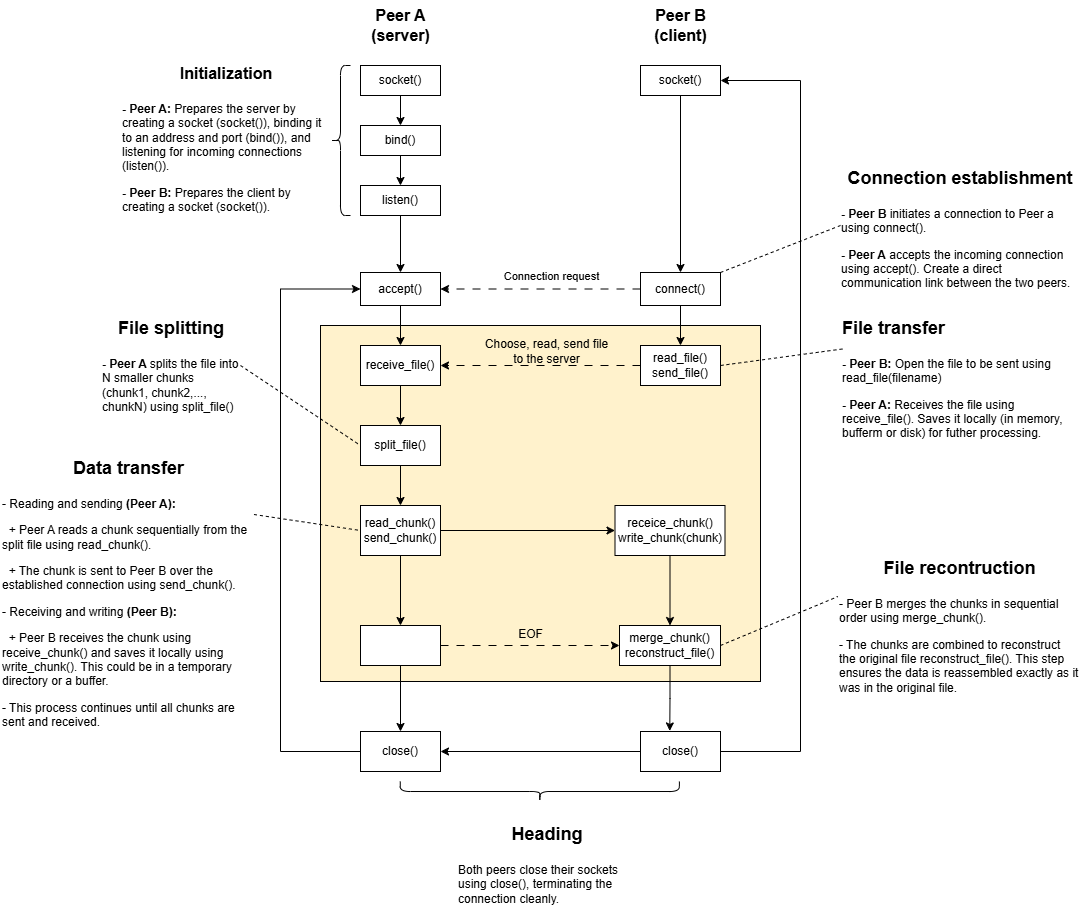
\includegraphics[width=\textwidth]{A-P2P-file-sharing-application-system.png}
    \caption{Illustration of Peer-to-Peer Network File Transfer Process}
    \label{fig:p2p-transfer}
\end{figure}

\section{Security Challenges}

\subsection{Overview}
Peer-to-peer (P2P) file sharing has revolutionized the way data is distributed by enabling direct file transfers between users without reliance on central servers. However, the decentralized nature of P2P networks also presents significant security risks and operational challenges.

\vspace{1em}
\noindent Security concerns include data corruption, malware distribution, and privacy risks due to unencrypted exchanges. Operationally, P2P networks face bandwidth strain, network instability, and difficulties in scaling effectively. They are also often associated with legal and ethical issues like copyright infringement.

\subsection{Security Issues in Peer-To-Peer File Sharing}

\begin{itemize}
    \item \textbf{Malware, Spyware and Viruses}: Since P2P networks allow direct sharing between users, files shared within the network may contain malware or viruses. These types of malicious software can cause all sorts of havoc, including bringing down your entire network. 
    \item \textbf{Data Integrity and Corruption}: Without a central authority to validate files, there is a risk of data corruption or unauthorized alterations. Users may unknowingly download corrupted files or altered versions of original files.
    \item \textbf{Privacy Risks}: Many P2P systems lack encryption for the files being exchanged. This exposes sensitive data to potential eavesdropping or interception. Users may unknowingly share personal or confidential information if the network is not adequately protected.
    \item \textbf{Insecurity File Transfer}: In some cases, P2P users may not be fully anonymous. IP addresses and activity logs can be traced back to users, leading to privacy breaches and potential legal consequences.
\end{itemize}

\subsection{Operational Challenges}

\begin{itemize}
    \item \textbf{Network Instability}: P2P networks often rely on user nodes that may join or leave at any time, causing fluctuations in the network’s availability and reliability. This can affect the quality and speed of file sharing.
    \item \textbf{Scalability}: As the network grows in size, managing the increasing number of peers and ensuring efficient file distribution becomes more difficult. P2P systems may face issues in scaling efficiently, leading to slower file sharing and connectivity problems.
    \item \textbf{Bandwidth Strain}: P2P networks often require users to share their internet bandwidth, which can lead to congestion and slow speeds, especially for users with limited bandwidth. This could affect the overall user experience.
    \item \textbf{Legal and Ethical Issues}: P2P networks are often used for sharing copyrighted content without authorization, leading to legal challenges. Copyright infringement lawsuits and ethical debates about file sharing in the context of intellectual property can complicate the use of P2P systems.
\end{itemize}

\subsection{Solutions and Mitigations}
\begin{itemize}
    \item \textbf{Encryption and Secure Protocols}: Implementing encryption at both the file and transport levels can mitigate the risks of data interception and malware. Protocols like TLS or SSL can be used to ensure the privacy and integrity of file transfers.
    \item \textbf{Authentication and Trust Models}: Introducing methods of verifying the identity of peers, such as digital signatures or reputation systems, can help prevent malicious actors from exploiting the network. Users can be rated or verified, increasing trust in the file-sharing process.
    \item \textbf{Legal Compliance and Content Filtering}: To avoid legal issues, some P2P networks implement content filtering and compliance with copyright laws, preventing the sharing of pirated content. This approach can help protect users from lawsuits and reduce the legal risk associated with file sharing.
    \item \textbf{Improved Network Protocols}: Enhancing network protocols to handle dynamic nodes more effectively and ensure more reliable peer discovery and file retrieval is crucial for overcoming scalability and stability challenges.
\end{itemize}


\section{Application of P2P}

\subsection{Advantages and disadvantages of P2P}

\textbf{Advantages}
\begin{itemize}
    \item P2P networks do not require the use of servers.
    \item Each computer device is a separate user manager.
    \item P2P operations do not require any complex specialized knowledge.
    \item Home and small business environments are suitable for using P2P networks.
    \item Does not require too much traffic when accessing the network.
\end{itemize}

\textbf{Disadvantages}
\begin{itemize}
    \item Information on the device cannot be backed up centrally.
    \item If multiple computer devices access at the same time, it will reduce performance.
    \item Data sets are not scientifically arranged but are stored on personal computers. This significantly affects the process of determining their location.
    \item Only providing some basic rights, poor security.
\end{itemize}

\subsection{Real-World Applications of P2P}

\begin{enumerate}
    \item File sharing: P2P is widely used to share files such as music files, videos, etc. The most typical application is Spotify's application so that users can search and save their favorite music. In more detail, Spotify has applied P2P network structure.
    
    \item Cryptocurrency: The basis of prominent cryptocurrencies such as Bitcoin is blockchain technology. Transactions all use the P2P network to authenticate transactions and maintain some decentralization. P2P technology ensures equality and transparency in financial transactions.
    
    \item Internet of Things (IoT): P2P is a technology that communicates directly between devices without relying on a central server. Therefore, P2P allows for faster data transmission and reduced latency in IoT applications.
\end{enumerate}

\subsection{Future Applications of P2P}

\begin{enumerate}
    \item Data sharing and privacy: P2P will improve and develop more in terms of security, while strengthening data control. This helps individuals manage their assets more effectively.
    
    \item Edge computing: P2P has the potential in edge computing, allowing devices at the edge of the network to communicate and collaborate effectively. P2P technology can improve the performance and scalability of edge computing applications by distributing computing resources and data processing.
    
    \item Collaborative Workspace: P2P technology can create a private network within the workspace by allowing secure and efficient resource sharing among distributed teams. Create a secure and highly productive collaborative workspace.
\end{enumerate}


\section{References}
\begin{itemize}
    % 1-introduction
    \item \href{https://www.geeksforgeeks.org/peer-to-peer-p2p-architecture/#what-is-a-peertopeer-p2p-architecture}{geeksforgeeks.org}

    % 2-architecture
    \item \href{https://example.com/napster}{Napster: The First Peer-to-Peer File Sharing Service.}

    \item \href{https://example.com/gnutella}{Gnutella Protocol Specification. }
    
    \item{chord Stoica, I., Morris, R., Karger, D., Kaashoek, M. F., \& Balakrishnan, H. (2001). Chord: A scalable peer-to-peer lookup protocol for internet applications. Proceedings of the 2001 conference on Applications, technologies, architectures, and protocols for computer communications.}
    
    \item \href{https://ipfs.io/}{IPFS: The InterPlanetary File System.}
    
    \item \href{https://bitcoin.org/bitcoin.pdf}{Nakamoto, S. (2008). Bitcoin: A Peer-to-Peer Electronic Cash System.}
    
    \item\href{https://webrtc.org/}{WebRTC: Enabling Real-Time Communications in Browsers.}
    
    \item \href{https://example.com/blockchain_p2p}{P2P Networks and Blockchain: Overview and Innovations.}


    % 3-transfer process
    \item \href{https://www.brosix.com/blog/peer-peer-file-transfer/}{Brosix: Peer-to-Peer File Transfer}
    \item \href{https://www.geeksforgeeks.org/p2p-peer-to-peer-file-sharing/}{GeeksforGeeks: P2P File Sharing}
    \item \href{https://www.raysync.io/news/everything-you-need-to-know-about-point-to-point-transfer/}{Raysync: Point-to-Point Transfer}
    \item Andrew S. Tanenbaum, "Computer Networks," 5th Edition.
    \item BitTorrent Protocol Specification.
    \item Peer-to-Peer Network Design and Applications.

    % 4-security
    \item \href{https://www.caplinked.com/blog/is-peer-to-peer-file-sharing-safe/}{Caplinked: How save is Peer-To-Peer File Sharing}
    \item \href{https://www.itsc.cuhk.edu.hk/it-policies/risks-in-peer-to-peer-file-sharing/}{CUHK-Information Technology Services Centre: Risk in Peer-To-Peer File Sharing}
    \item \href{https://www.securedocs.com/blog/2013/02/peer-to-peer-p2p-file-sharing-risks}{SecureDocs: Peer-To-Peer (P2P) File Sharing Risks}

    
\end{itemize}

\end{document}
